\documentclass[../../main.tex]{subfiles} % Allows individual compilation
\graphicspath{{\subfix{../../images/}}}

\begin{document}

\section{Observations préliminaires}

\subsection{Décomposition de la matrice d'adjacence} 
C'est toujours possible de décomposer une matrice comme la somme de son 
espérance (qui est déterministe) et une matrice aléatoire de ``résidus'':
\[
	\frac{1}{\sqrt{n}} A = \frac{1}{\sqrt{n}} \left( \mathbb E 
	\left[ A \right] + V \right).
\]
Il faut alors démontrer les propriétés de l'énoncé. Etablissons d'abord une 
notation qui nous sera utile. Notons que
\begin{equation}
	\mathbb E \left[ A \right]_{ij} = \mathbb E \left[ A_{ij} \right] 
	= q_i q_j C_{ab}
	\label{eq:decompA}
\end{equation}
Soit $Q = \diag q$ et $J \in \R{n \times K}$ une matrice telle que $J_{ij} 
= \delta_{i \in \mathcal{C}_j}$. Soit aussi $C \in \R{K \times K}$ la matrice 
des $C_{ab}$. Alors, definissons une matrice ``augmentée'' $C^A \in 
\R{n \times n}, C^A := JCJ^t$. Cette matrice est telle que 
$\left(C^A \right)_{ij} = C_{ab}$ si $i \in \mathcal{C}_a$ et 
$j \in \mathcal{C}_b$. Alors nous pouvons écrire
\begin{equation*}
	\frac{1}{\sqrt n} A = \frac{1}{\sqrt n} \left( Q C^A Q + V \right)
\end{equation*}
Nous pouvons aussi développer cela en fonction de la matrice $M$, car 
$C = \ones{K \times K} + M/ \sqrt n$. En utilisant le fait facilement vérifiable
que
\begin{equation}
	J \ones{K \times K} J^t = \ones{n \times n},
	\label{eq:ones}
\end{equation}
nous arrivons à
\begin{equation*}
	\frac{1}{\sqrt n} A = Q \left( \frac{\ones{n \times n}} {\sqrt n} 
	+ \frac{J M J^t }{n} \right) Q + \frac{V}{\sqrt n}.
\end{equation*}

\paragraph{Rang de la partie déterministe.} A un facteur $1/ \sqrt n$ près, la 
partie déterministe vaut $Q C^A Q$. En plus, $Q$ a rang plein (car c'est 
diagonale avec $q_i > 0$), alors $\rank{Q C^A Q} = \rank {C^A} = \rank{J C J^t}$.
Nous avons l'inégalité fondamentale pour toutes deux matrices $A, B$:
\begin{equation*}
	\rank{AB} \leq \min \left\{ \rank A, \rank B \right\},
\end{equation*}
alors, en utilisant le fait que $\rank J = \rank{J^t}$,
\begin{equation}
	\rank{J C J^t} \leq \min\left\{\rank J, \rank C\right\}.
\label{eq:rankdet}
\end{equation}
Or, les colonnes de $J$ représentent les clusters du graphe. En particulier, si
chaque point appartient à un seul cluster, alors une colonne n'est pas multiple
d'autre et on voit que $J$ a rang plein. Comme $J \in \R{n \times K}$, alors en
assumant que $n \geq K$, alors $\rank J = K$. Finalement, $C \in \R{K \times K}$
implique $\rank C \leq K$. Alors l'équation \ref{eq:rankdet} devient
\[
\rank{J C J^t} \leq K.
\]
d'où le rang de la partie déterministe de $A / \sqrt n$ est au plus $K$.

\paragraph{Analyse de la partie aléatoire.} Comme les entrées $A_{ij}$ étaient 
indépendantes, alors $V = A - \esp A$ a entrées indépendantes aussi, cas 
substraire des constantes ne modifie pas la dépendance des entrées. Nous 
vérifions facilement que $V$ a entrées centrées:
\begin{equation*}
	\esp{V_{ij}} = \esp{A_{ij} - \esp{A_{ij}}} = 0.
\end{equation*}
Une analyse similaire peut être réalisée pour la variance:
\begin{equation}
	\esp{V_{ij}^2} = \esp{ \left( A_{ij} - \esp{A_{ij}}\right)^2} 
	= \var{A_{ij}} = q_i q_j C_{ab} \left( 1 - q_i q_j C_{ab} \right)
	\label{eq:variance}
\end{equation}
Il nous sera utile (pour prendre la limite $n \to \infty$) de noter que cette 
équation peut être écrite, après une simple expansion des termes, comme
\begin{equation*}
	\esp{V_{ij}^2} = q_i q_j \left( 1 - q_i q_j \right) + \mathcal{O} 
	\left( \frac{1}{\sqrt n} \right).
\end{equation*}

\subsection{Décomposition de la matrice de modularité} 
Etant donnée la décomposition de la matrice d'adjacence, on obtient une 
décomposition de la matrice de modularité $B/ \sqrt n = A - q q^t$. Notons que 
$q q^t = Q \ones{n \times n} Q$, alors
\begin{equation*}
	\frac{B}{\sqrt n} = \frac{Q \left( C^A - \ones{n \times n}\right) Q}
	{\sqrt n} + \frac{V}{\sqrt n}.
\end{equation*}
Cette même expression peut être écrite en termes de $M$:
\begin{equation*}
	\frac{B}{\sqrt n} = Q \left( \frac{J \ones{K \times K} J^t}{\sqrt n} 
	+ \frac{J M J^t}{n} - \frac{\ones{n \times n}}{\sqrt n} \right) Q 
	+ \frac{V}{\sqrt n}
\end{equation*}
En utilisant l'équation \ref{eq:ones}, on obtient
\begin{equation}
	\frac{B}{\sqrt n} = \frac{Q J M J^t Q}{n} + \frac{V}{\sqrt n}.
	\label{eq:B}
\end{equation}
Cette équation nous permet de faire l'interprétation suivante: la matrice $M$ 
représente la densité des clusters. Si une entrée $M_{ii} \gg 1$, alors le 
cluster $i$ est très dense et donc ``plus facile'' à identifier. Comme dans les
spiked models, cela peut être interprété comme un signal fort. Par contre, si 
$M_{ii} \ll 1$, alors le cluster $i$ n'est pas trop dense et donc plus difficile 
à détecter. En analogie aux spiked models, cela serait un signal faible. La 
partie aléatoire $V/\sqrt n$, après due normalisation, a son spectre tendant 
vers une loi du semi-cercle, et cela représenterait du bruit.

\subsection{Représentation graphique des valeurs et vecteurs propres}
Représentons graphiquement le spectre de $B / \sqrt n$ pour des différents 
choix de $M$ et $q_i$.

\paragraph{Premier cas.} Nous prenons $q_i = q_0 = 0.05$ pour tout $i$. Cela 
signifie que tout noeud dans le graphe a le même prior de connectivité. On 
dénote par $M \sim \mu$ le fait d'avoir $M_{ii} \sim U\left(0, \mu \right), 
\forall i$. On prendra $n = 3000$ et $M \sim 100, 500, 1000$. Cela correspond 
à avoir l'ordre de $M$ étant d'ordre égale à $\sqrt{n}$, entre $\sqrt n$ et $n$,
égale à $n$, respectivement. On prendra aussi des communautés symmétriques, 
c'est-à-dire, le nombre de points dans chaque communauté sera le même en moyenne.
Les spectres trouvés ainsi que leurs vecteurs propres sont organisés à la Figure 
\ref{fig:spectres_prelim_1}. 
Nous observons que quand $M$ est petite, alors le spectre n'a pas de spikes et 
ressemble à une loi du semi-cercle. Cela arrive car dans ce cas la partie
aléatoire de $A/\sqrt n$ sera une matrice de Wigner.
Lorsque $M$ croît, on observe le nombre de spikes augmenter. Le nombre de 
valeurs propres isolées va jusqu'à trois, ce qui est d'accord avec l'observation
d'avoir le rang de la partie déterministe de $A$ inférieur ou égal à $K=3$.
Nous observons que quand $M$ est suffisament grand pour que le spectre ait des 
spikes, alors les vecteurs propres s'approchent des vecteurs canoniques. Quand 
l'ordre de $M$ diminut, alors les vecteurs propres deviennent moins distingués.

\begin{figure}
	\begin{tabular}{cc}
		% M ~ 1000
		\subfloat[$M \sim 1000$ (eigenvalues)]{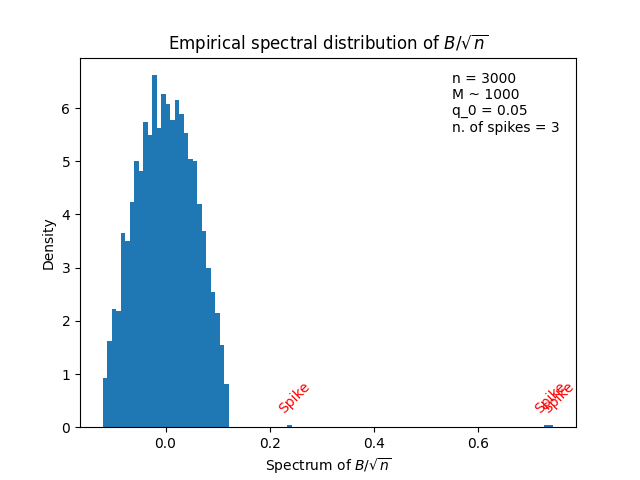
\includegraphics[width=0.5\textwidth]{../../images/observations_preliminaires/case_1/M_1000/spectrum.png}} &
		\subfloat[$M \sim 1000$ (eigenvectors)]{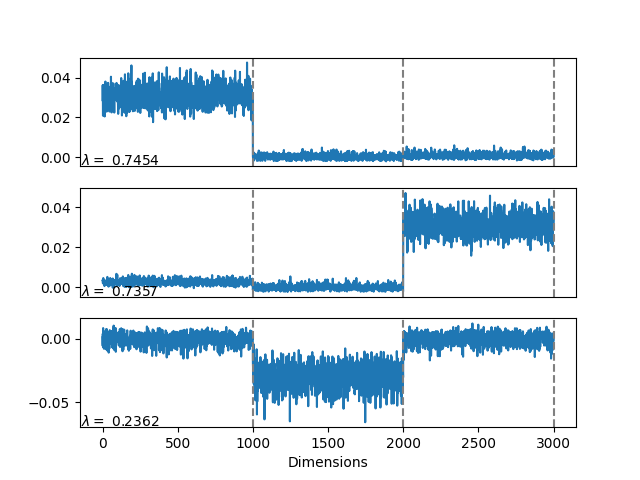
\includegraphics[width=0.5\textwidth]{../../images/observations_preliminaires/case_1/M_1000/eigenvectors.png}} \\
		% M ~ 500
		\subfloat[$M \sim 500$ (eigenvalues)]{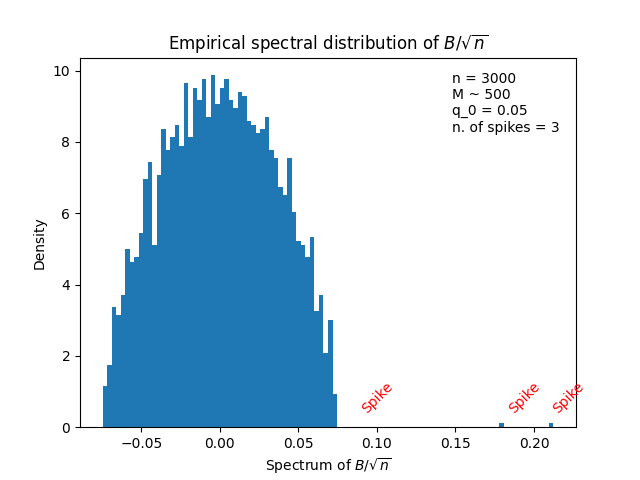
\includegraphics[width=0.5\textwidth]{../../images/observations_preliminaires/case_1/M_500/spectrum.png}} &
		\subfloat[$M \sim 500$ (eigenvectors)]{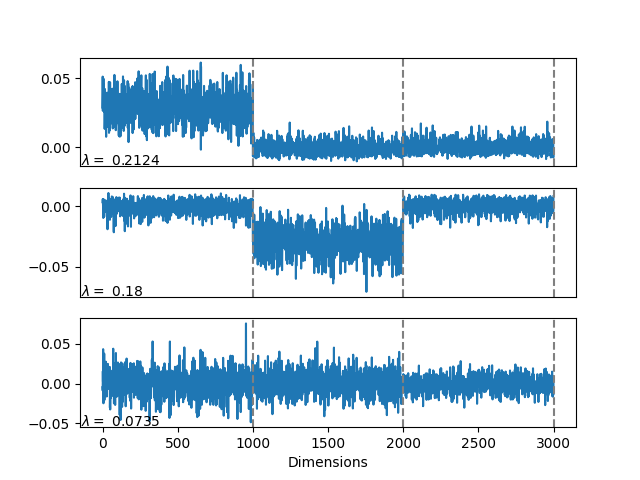
\includegraphics[width=0.5\textwidth]{../../images/observations_preliminaires/case_1/M_500/eigenvectors.png}} \\
		% M ~ 100
		\subfloat[$M \sim 100$ (eigenvalues)]{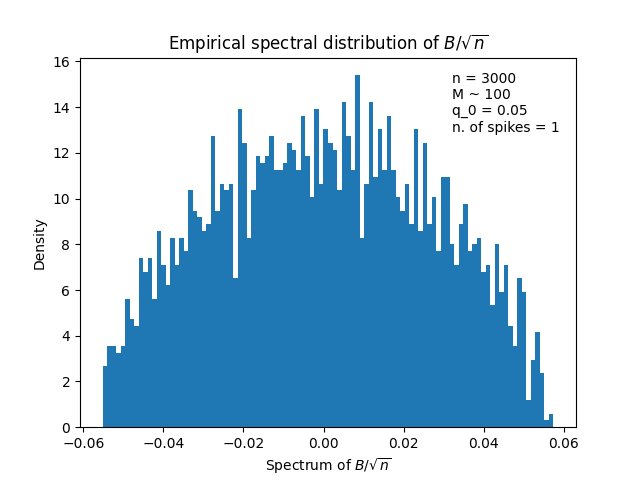
\includegraphics[width=0.5\textwidth]{../../images/observations_preliminaires/case_1/M_100/spectrum.png}} &
		\subfloat[$M \sim 100$ (eigenvectors)]{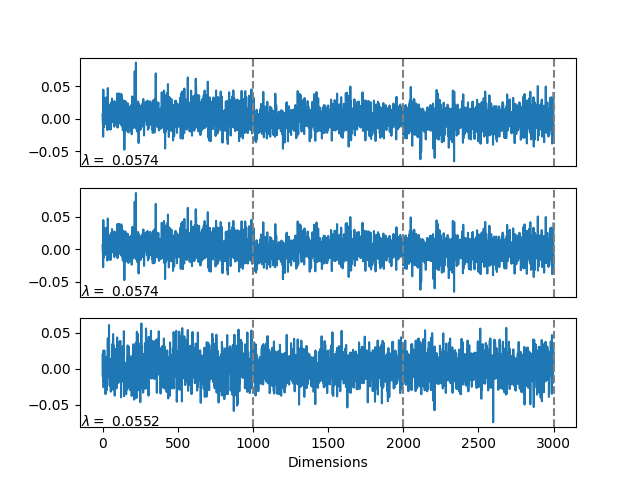
\includegraphics[width=0.5\textwidth]{../../images/observations_preliminaires/case_1/M_100/eigenvectors.png}} \\
	\end{tabular}
	\caption{Spectre et vecteurs propres dans le cas homogène pour des 
	différentes valeurs de $M$}
	\label{fig:spectres_prelim_1}
\end{figure}

\paragraph{Deuxième cas.} Maintenant nous considérons $q_i$ uniforme autour de 
$q_0 = 0.5$, avec une fênetre de taille $0.25$. Nous avons testé les valeurs 
$M \sim 1, 10, 50$ dans ce cas. Le spectre observé, ainsi que les vecteurs 
propres associés, sont montrés à la Figure \ref{fig:spectre_prelim_2}. Comme 
avant, $M$ plus grand implique des spikes et des vecteurs propres plus définis
et proches des vecteurs canoniques des classes.

\begin{figure}
	\begin{tabular}{cc}
		% M ~ 50
		\subfloat[$M \sim 50$ (eigenvalues)]{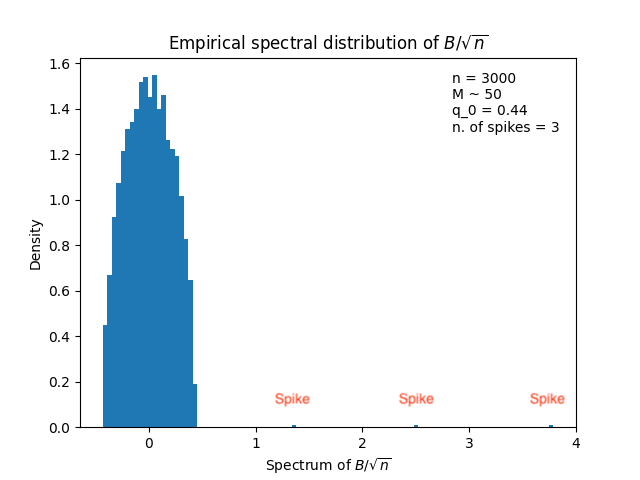
\includegraphics[width=0.5\textwidth]{../../images/observations_preliminaires/case_2/M_50/spectrum.png}} &
		\subfloat[$M \sim 50$ (eigenvectors)]{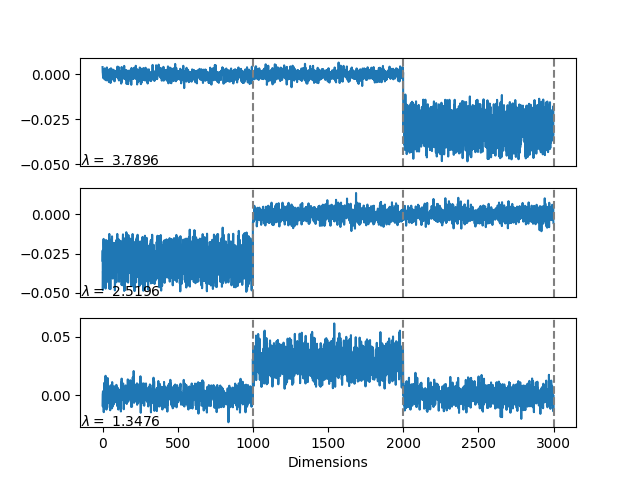
\includegraphics[width=0.5\textwidth]{../../images/observations_preliminaires/case_2/M_50/eigenvectors.png}} \\
		% M ~ 10
		\subfloat[$M \sim 10$ (eigenvalues)]{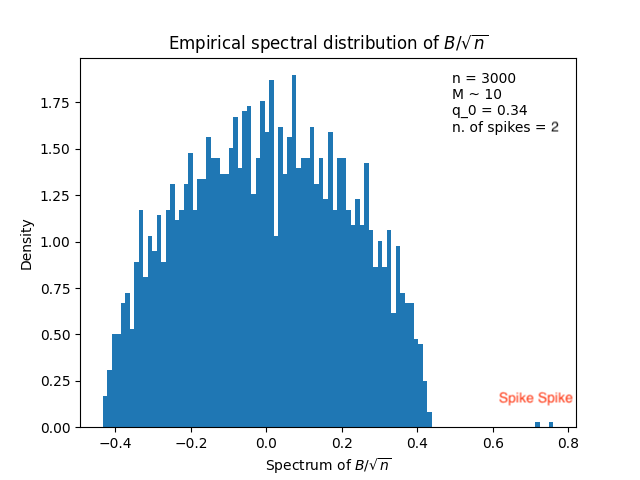
\includegraphics[width=0.5\textwidth]{../../images/observations_preliminaires/case_2/M_10/spectrum.png}} &
		\subfloat[$M \sim 10$ (eigenvectors)]{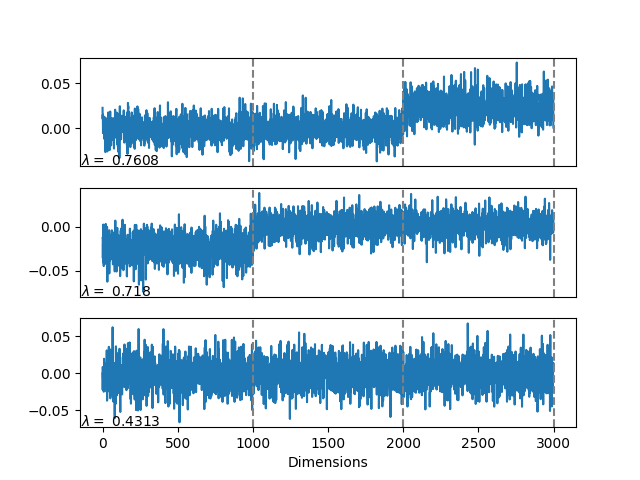
\includegraphics[width=0.5\textwidth]{../../images/observations_preliminaires/case_2/M_10/eigenvectors.png}} \\
		% M ~ 1
		\subfloat[$M \sim 1$ (eigenvalues)]{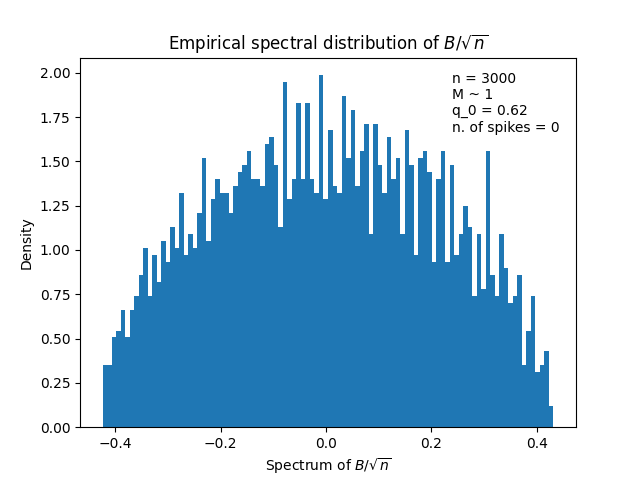
\includegraphics[width=0.5\textwidth]{../../images/observations_preliminaires/case_2/M_1/spectrum.png}} &
		\subfloat[$M \sim 1$ (eigenvectors)]{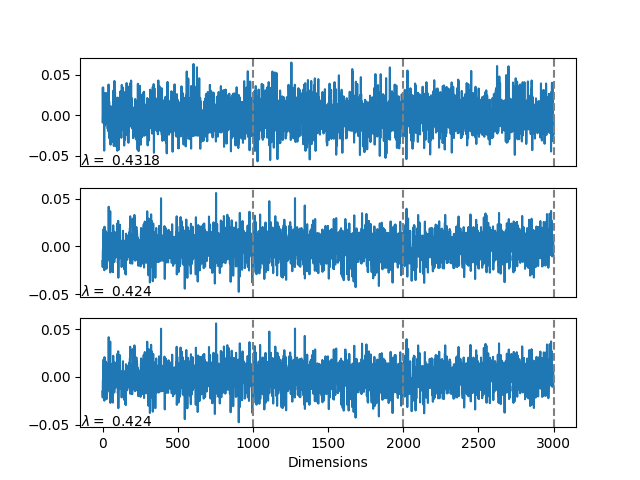
\includegraphics[width=0.5\textwidth]{../../images/observations_preliminaires/case_2/M_1/eigenvectors.png}}
	\end{tabular}
	\caption{Spectre dans le cas $q_i \sim U\left(0.25, 0.75\right)$, pour 
	des différentes valeurs de $M$}
	\label{fig:spectre_prelim_2}
\end{figure}

\paragraph{Troisième cas.} Maintenant nous considérons $q_i \in \left\{ q^{(1)},
q^{(2)} \right\}$ pour deux valeurs très différentes: $q^{(1)}=0.5$ et $q^{(2)}
=0.05$. Nous avons testé les valeurs $M \sim 10, 50, 100$ dans ce cas. Le spectre 
observé est montré à la Figure \ref{fig:spectre_prelim_3}. Curieusement, la 
distribution limite ne semble pas être une loi du semi-cercle. Les vecteurs 
propres pour $M$ grand oscillent autour de zéro dehors la classe correspondante
à eux, mais sur la partie de la classe correcte ils sont très bruités.

\begin{figure}
	\begin{tabular}{cc}
		% M ~ 100
		\subfloat[$M \sim 100$ (eigenvalues)]{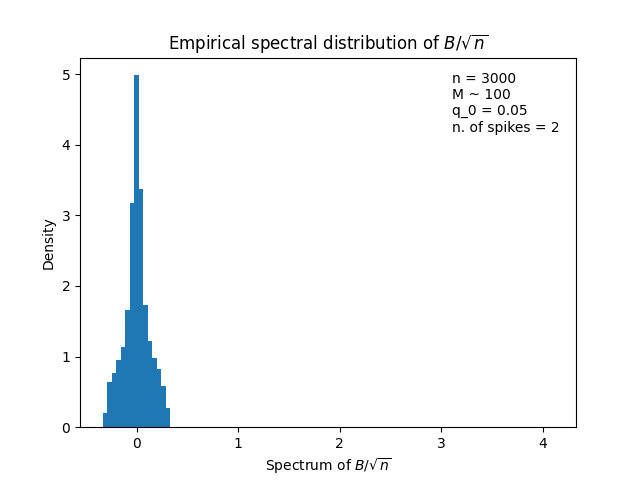
\includegraphics[width=0.5\textwidth]{../../images/observations_preliminaires/case_3/M_100/spectrum.png}} &
		\subfloat[$M \sim 100$ (eigenvectors)]{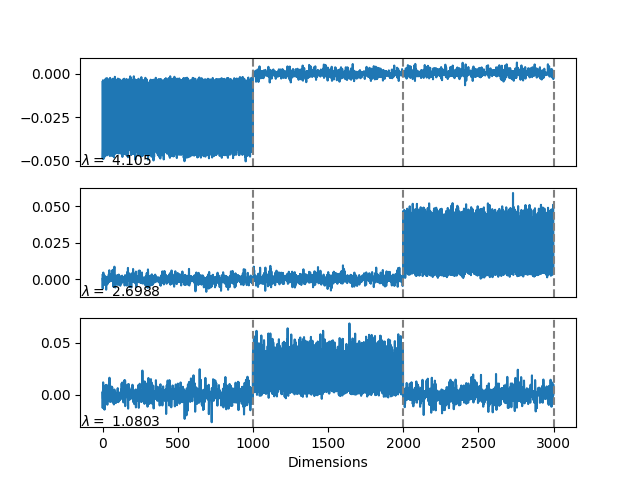
\includegraphics[width=0.5\textwidth]{../../images/observations_preliminaires/case_3/M_100/eigenvectors.png}} \\
		% M ~ 50
		\subfloat[$M \sim 50$ (eigenvalues)]{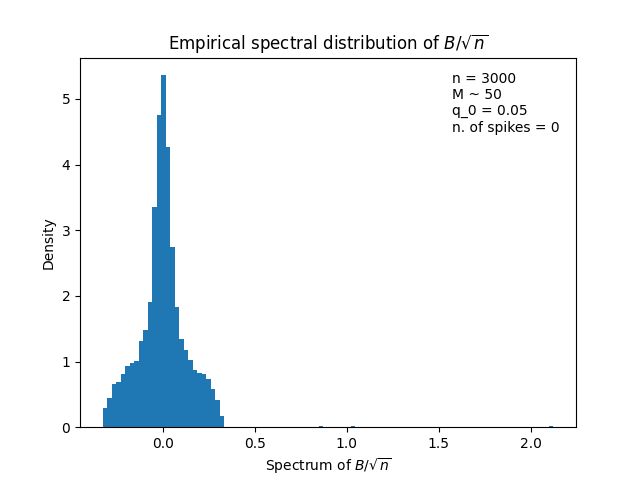
\includegraphics[width=0.5\textwidth]{../../images/observations_preliminaires/case_3/M_50/spectrum.png}} &
		\subfloat[$M \sim 50$ (eigenvectors)]{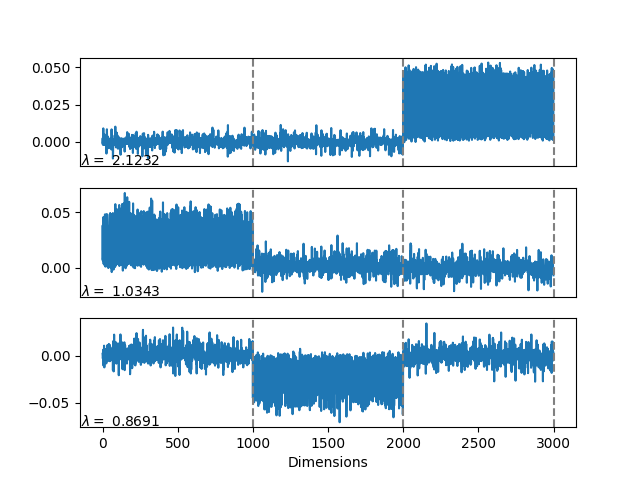
\includegraphics[width=0.5\textwidth]{../../images/observations_preliminaires/case_3/M_50/eigenvectors.png}} \\
		% M ~ 10
		\subfloat[$M \sim 10$ (eigenvalues)]{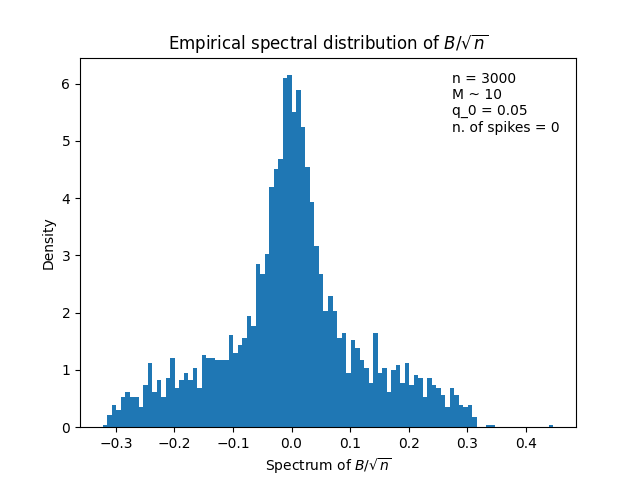
\includegraphics[width=0.5\textwidth]{../../images/observations_preliminaires/case_3/M_10/spectrum.png}} &
		\subfloat[$M \sim 10$ (eigenvectors)]{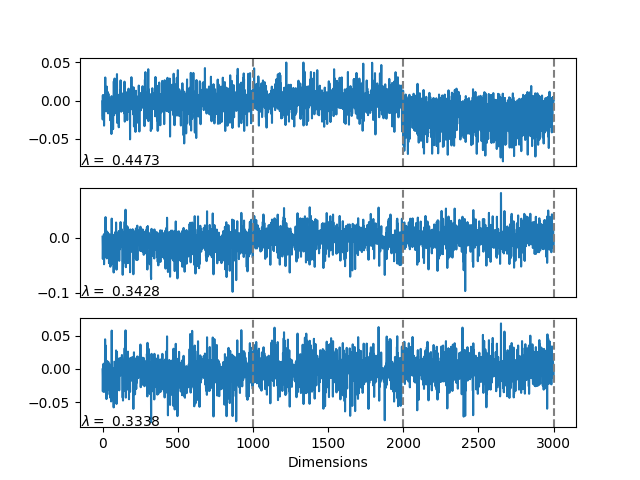
\includegraphics[width=0.5\textwidth]{../../images/observations_preliminaires/case_3/M_10/eigenvectors.png}}
	\end{tabular}
	\caption{Spectre dans le cas $q_i \in \left\{ 0.05, 0.5 \right\}$, pour 
	des différentes valeurs de $M$}
	\label{fig:spectre_prelim_3}
\end{figure}

\end{document}
